\documentclass[11pt,nswissgerman]{article}
\usepackage{helvet}
\renewcommand{\familydefault}{\sfdefault}
\usepackage[latin2]{inputenc}
\usepackage[a4paper]{geometry}
\geometry{verbose,tmargin=3cm,bmargin=3cm,lmargin=3.5cm,rmargin=3.5cm,headheight=3cm,headsep=1cm,footskip=2cm}
\usepackage{fancyhdr}
\pagestyle{fancy}
\usepackage{wrapfig}
\usepackage{graphicx}
\usepackage[position=bottom]{subfig}
\usepackage{titletoc}
\usepackage{float}
\makeatletter
\usepackage[T1]{fontenc}
\@ifundefined{date}{}{\date{}}
\makeatother
\usepackage{babel}
\usepackage[
            colorlinks=true,
            urlcolor=green,
            linkcolor=black
]{hyperref}
\setcounter{secnumdepth}{1} % levels under \section are not numbered
\setcounter{tocdepth}{2}    % levels under \subsection are not listed in the TOC
\begin{document}
\author{Stefan Bopp}
\title{\Huge Tagebuch Bretagne 2016\vspace{2cm}

\includegraphics[width=0.4\textwidth]{../Bilder/Logo/Logo.png}
}
\maketitle
\vfill
\tableofcontents

\newpage

\lhead{Bretagne 2016}

\rhead{jackthebus.com}

\cfoot{\thepage}
%    JJJ    AA     CCCCCC KKK   K TTTTTT HH  HH EEEEEE BBBBBB UU  UU SSSSSS    CCCCCC OOOOOO MM  MM
%    JJJ   AAAA    CCCCCC KKK  K  TTTTTT HH  HH EEEEEE BB   B UU  UU SSS       CCCCCC OOOOOO MM  MM
%    JJJ  AA  AA   CC     KKK K     TT   HHHHHH EEE    BB   B UU  UU SSS       CC     OO  OO MMMMMM
%    JJJ AA    AA  CC     KKKK      TT   HHHHHH EEEEEE BBBBBB UU  UU  SSSSS    CC     OO  OO M MM M
%    JJJ AAAAAAAA  CC     KKK K     TT   HH  HH EEE    BB   B UU  UU    SSS    CC     OO  OO M MM M
% JJJJJJ AA    AA  CCCCCC KKK  K    TT   HH  HH EEEEEE BB   B UUUUUU    SSS .. CCCCCC OOOOOO M MM M
% JJJJJJ AA    AA  CCCCCC KKK   K   TT   HH  HH EEEEEE BBBBBB UUUUUU SSSSSS .. CCCCCC OOOOOO M MM M
% 
% Texte Geschrieben von Stefan Bopp und Chantal Frunz
% Mehr Informationen sind auf jackthebus.com zu finden
%
\subsection{29.08.2016 - 02.09.2016 Vorbereitungen}

\begin{wrapfigure}{R}{0.45\textwidth} 
  \begin{centering}
    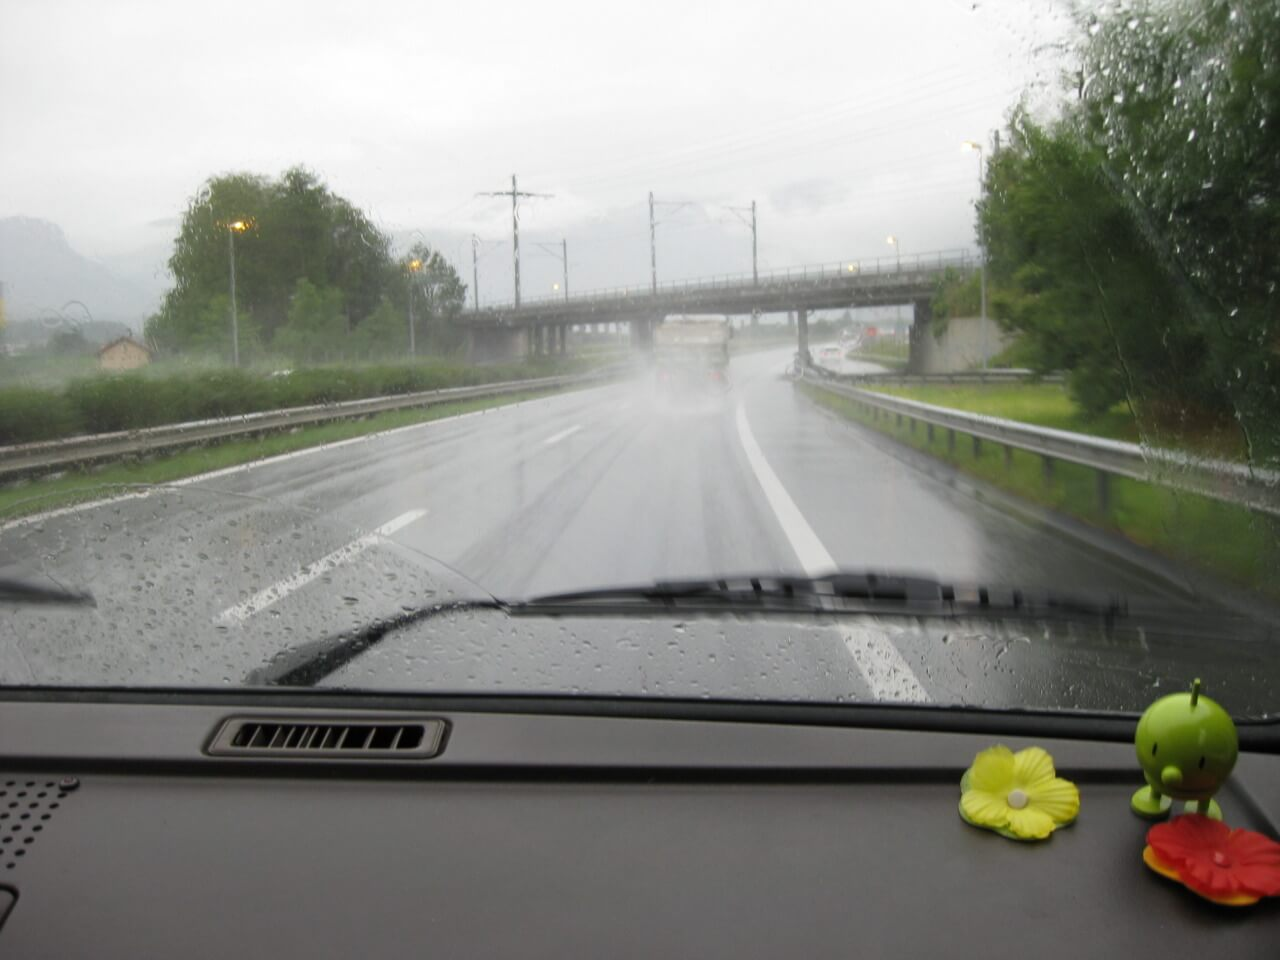
\includegraphics[width=0.4\textwidth, height=5cm, keepaspectratio]{../Bilder/Dolomiten/1.jpg}
    \caption{Regen}
  \end{centering}
\end{wrapfigure} 

\begin{figure}[b]
   \centering
      %\subfloat[CAPTION]{BILDERCODE}\qquad
   \subfloat{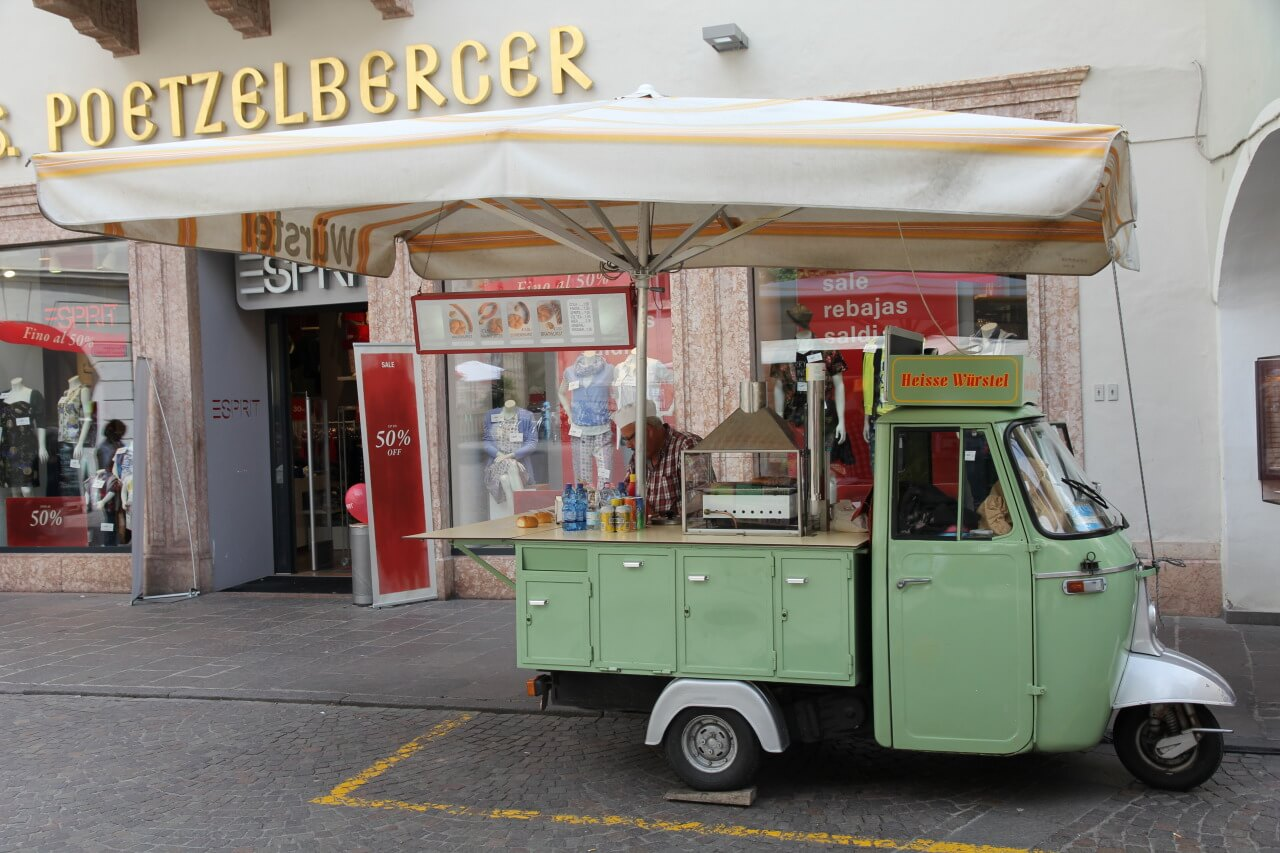
\includegraphics [width=0.3\textwidth]{../Bilder/Dolomiten/2.jpg}}\quad
   \subfloat{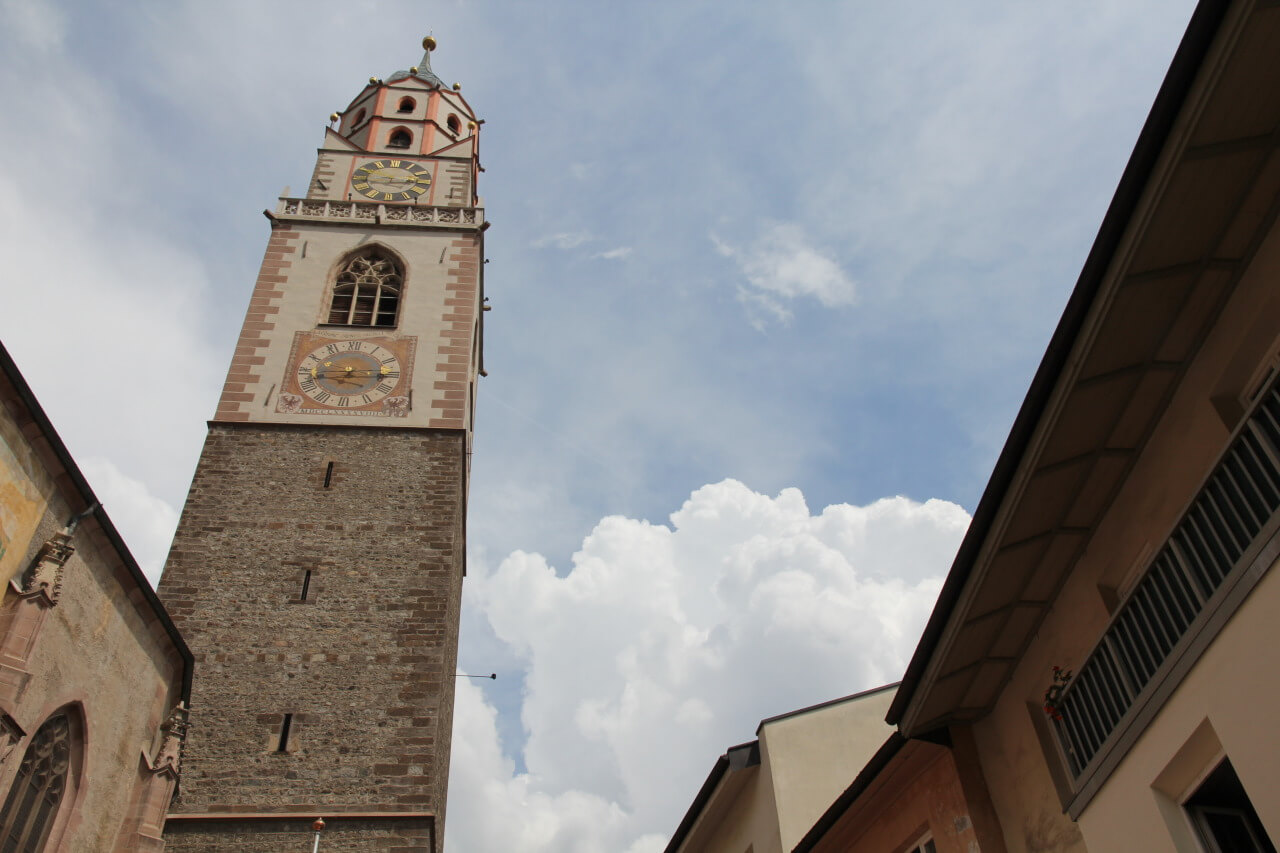
\includegraphics [width=0.3\textwidth]{../Bilder/Dolomiten/3.jpg}}\quad
   \subfloat{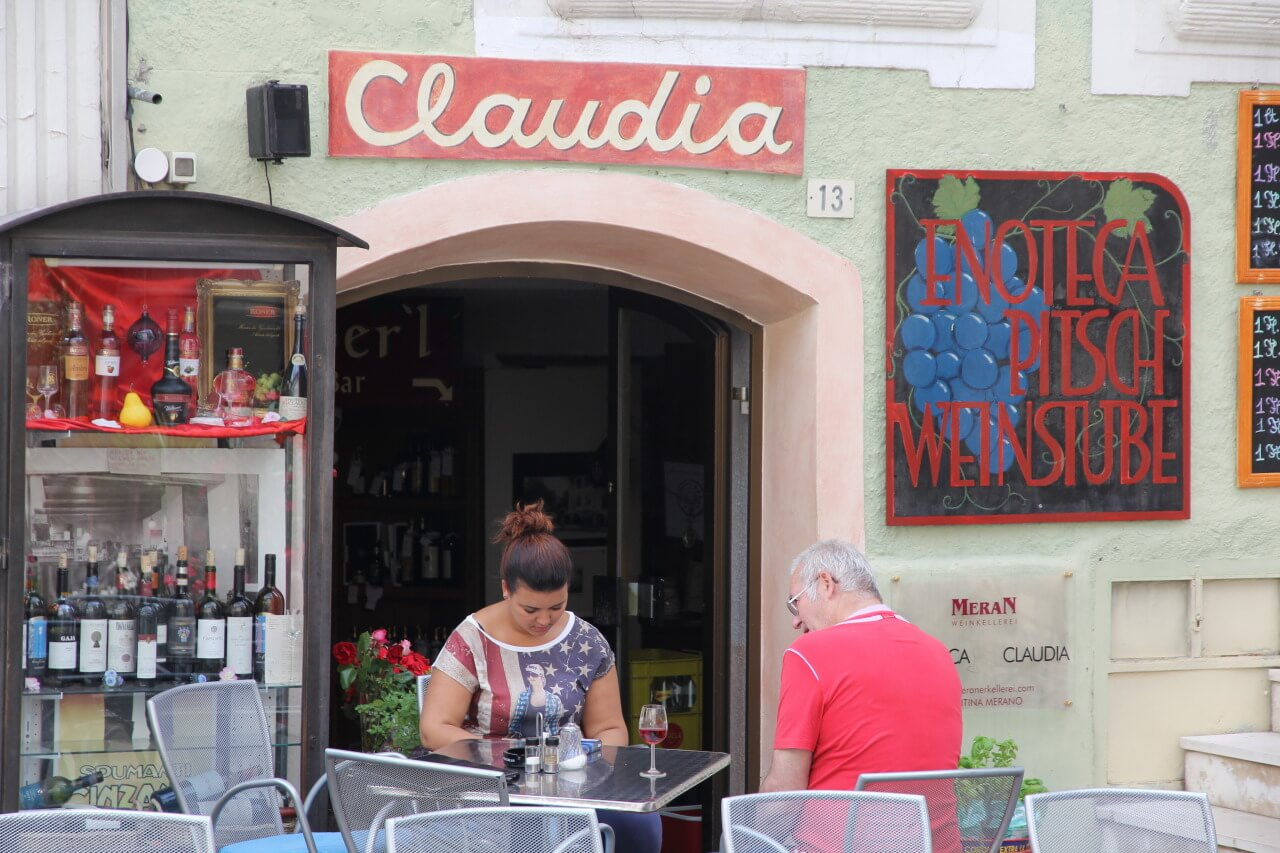
\includegraphics [width=0.3\textwidth]{../Bilder/Dolomiten/4.jpg}}\quad
   \caption[Meran]{Meran}
\end{figure}
>>>>>>> 10fde08af849bf090ad768de228b1b7e9c4373a7

Die Vorbereitungen zogen sich fast �ber eine Woche hin. Diverse Modifikationen und Reparaturen wurden am Bus durchgef�hrt. Eine kurze Auflistung dieser:

\begin{itemize}
    \item Schloss an der Schiebet�re ersetzt
    \item Tacho repariert
    \item Neuer Tisch eingebaut
    \item Massepunkt repariert
    \item Relais f�r Intervall Scheiben-Wischer eingebaut
    \item Packen f�r die bevorstehende Reise
    \item Vorbereiten des Autos
\end{itemize}

Alles in Allem ungef�hr eine gem�tliche Woche Arbeit, welche im H�henpunkt der Abfahrt am Samstag morgen endete.

\subsection{03.09.2016 Reise in die Bretagne}

\begin{figure}[b]
   \centering
      %\subfloat[CAPTION]{BILDERCODE}\qquad
   \subfloat{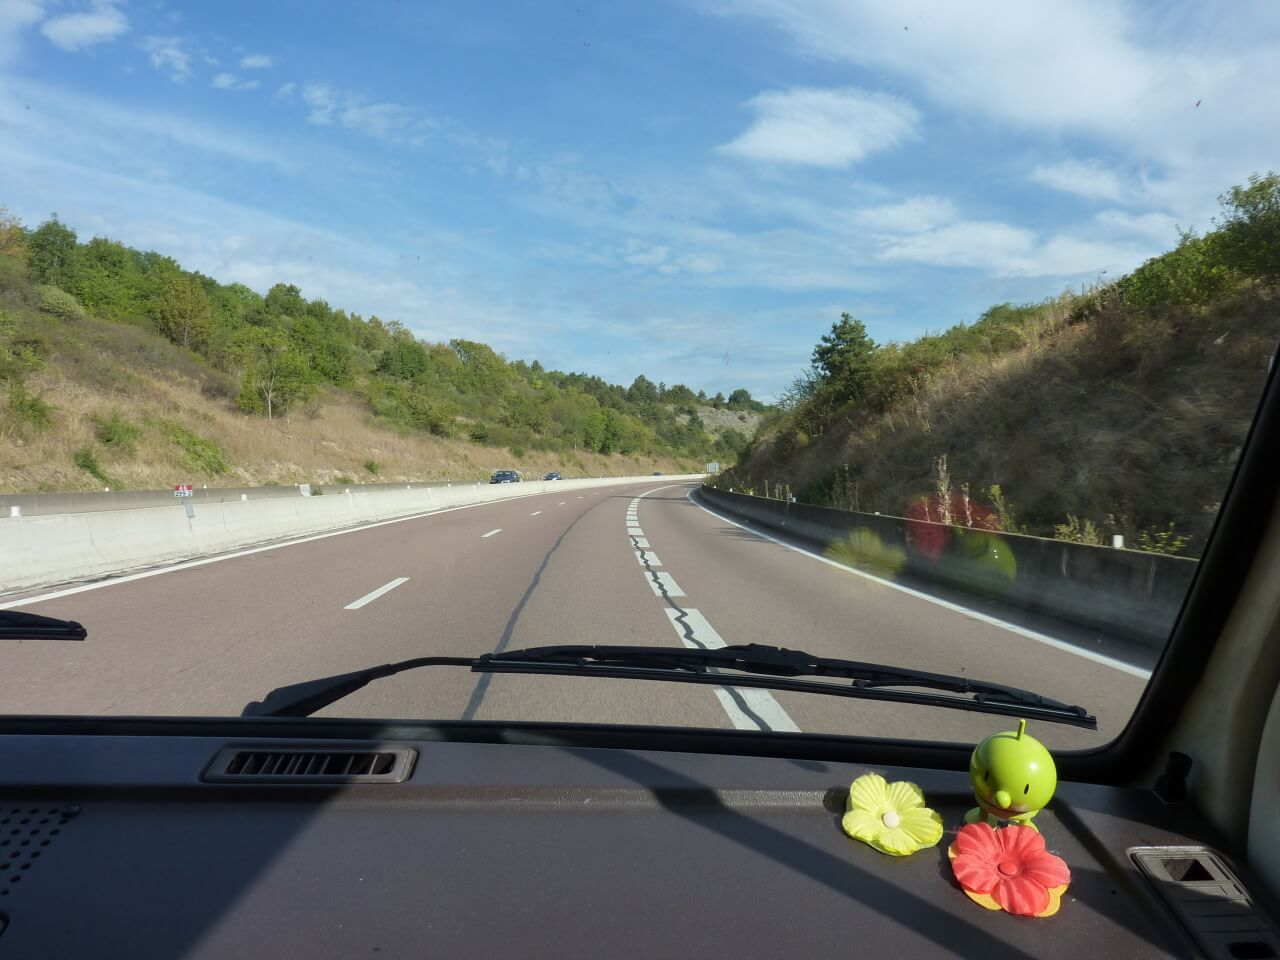
\includegraphics [width=0.3\textwidth]{../Bilder/Bretagne/1.jpg}}\quad
   \subfloat{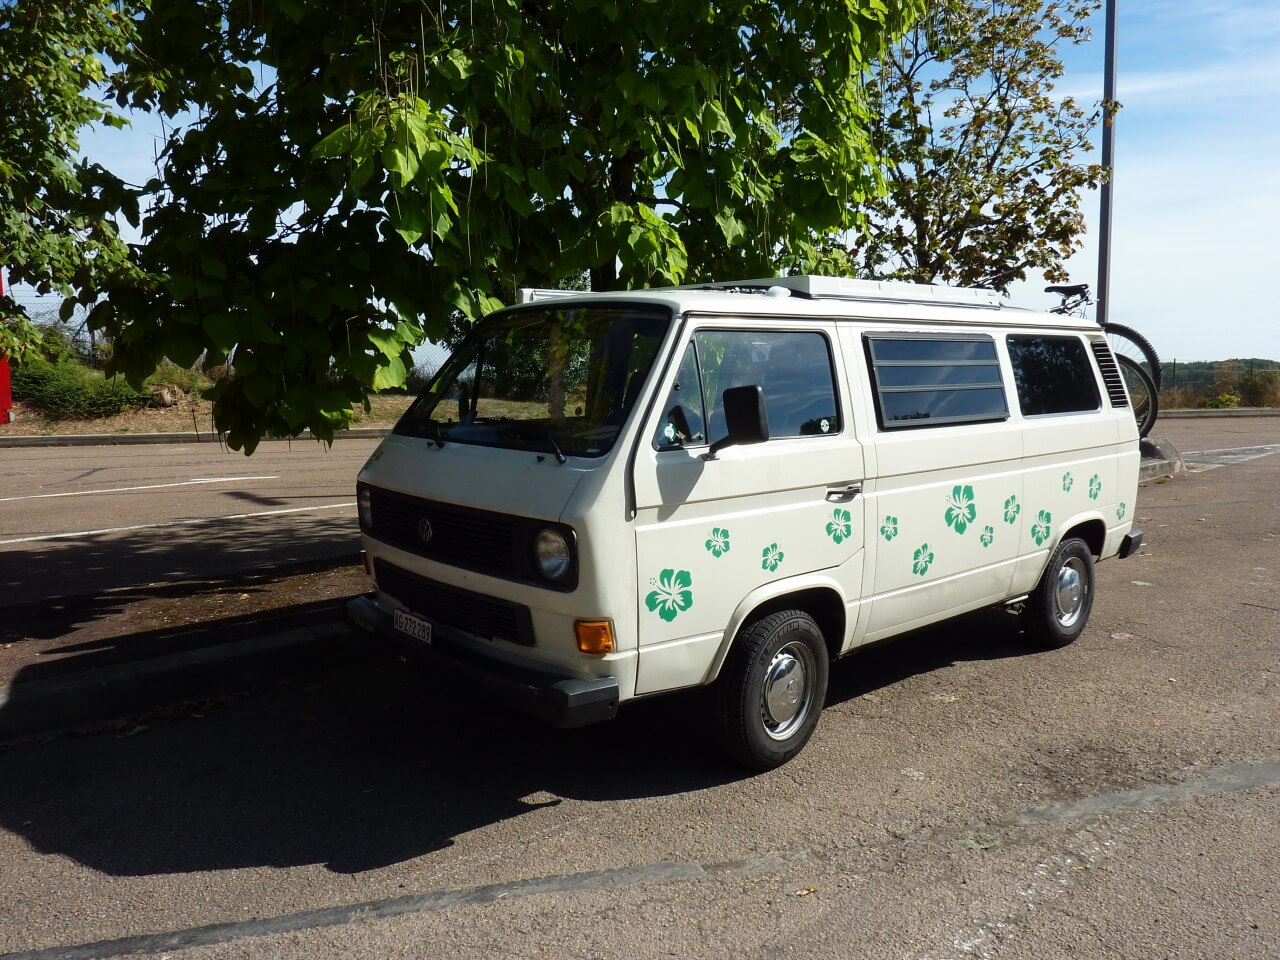
\includegraphics [width=0.3\textwidth]{../Bilder/Bretagne/2.jpg}}\quad
   \subfloat{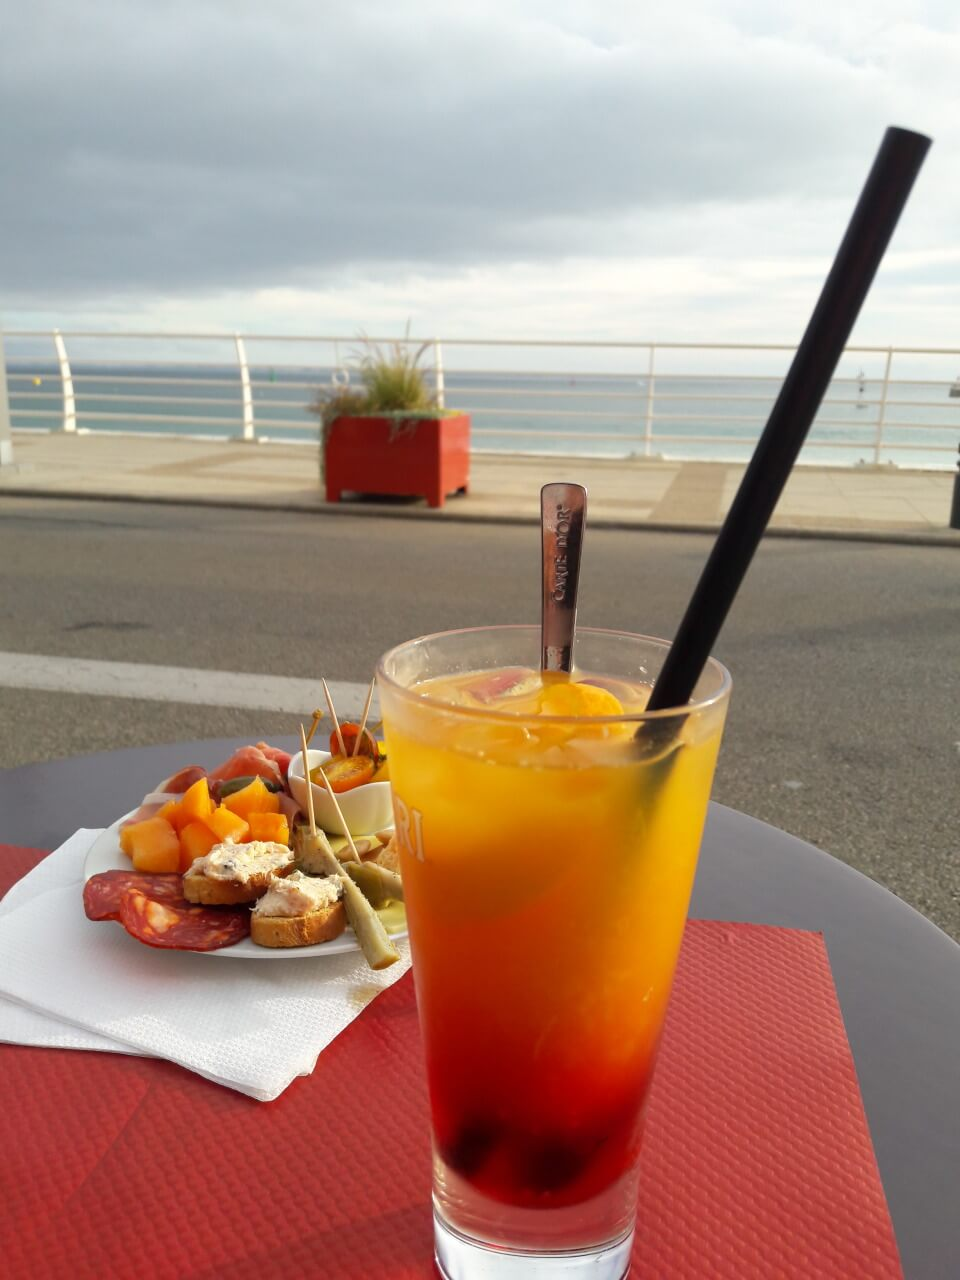
\includegraphics [width=0.17\textwidth]{../Bilder/Bretagne/3.jpg}}\quad
   \caption[Quiberon]{Quiberon}
\end{figure}

Fr�h um 04:00 klingelte der Wecker und l�utete damit eine neue Episode unserer Bus Reisen ein.
Trotz gewissen Zweifeln am Ziel, die Bretagne mit dem Bus zu bereisen haben wir uns schlussendlich dazu entschlossen, denn weiten Weg auf uns zu nehmen.
Etliche Reisef�hrer rieten davon ab den von Navigationsanbieter vorgeschlagenen Weg �ber Paris einzuschlagen.
Mittels selbst entworfener Route in google maps und dem Papier Ausdruck davon machten wir uns auf den Weg Richtung Basel.
Nach der dritten Kurve fiel zum ersten Mal das Radio aus, genauer gesagt beklagte sich der Batteriew�chter �ber eine zu tiefe Spannung und trennte die Verbraucherbatterie ab.
Schluss mit lustig, kein Radio, kein K�hlschrank\dots{}
Alles wieder eingeschaltet und weiter ginge es, jedoch nicht sehr weit.
Noch vor der Autobahneinfahrt entschied sich das autorit�re System ein weiteres Mal f�r ein black-out.

Auf der Rastst�tte hielten wir kurz an und ich begutachtete den \glqq Schaden\grqq{} unter dem Schein der Taschenlampe.
Beim Einbau des \glqq Battery Power Management System\grqq{} gab es ein kleines Missgeschick welches dazu f�hrte, dass der L�tkolben gez�ckt werden musste und einer der Verbindungen wollte den Vibrationen von Jack nicht Herr werden.
So kam es zum Einsatz des L�tkolbens um halb 5 und einer hoffentlich erfolgreichen Reparatur (Bis jetzt soweit ok).

Kurz nach der Grenze mussten wir laut der Routenbeschreibung die Autobahn verlassen und die Reise �ber das Netz von Schnellstrassen fortsetzten.
Nach 10 Minuten, zweite Ausfahrt jetzt, danach links abbiegen und Einfahrt in eine 30er Zone war es eine leichte Entscheidung einfach dem Navi zu vertrauen und die Navigation einem h�herem (GPS) System zu �berlassen, da wir selbst f�r die n�chsten paar Stunden als Chauffeur gefordert waren.


Nach mehreren Zahlstellen (kommt schon was zusammen) und etlichen Stunden Fahrt unterbrochen von Fahrerwechsel und Tankstopps, n�herten wir uns der Atlantikk�ste.
Die Fahrt verlief absolut ereignislos und teilweise eher langweilig durch die ewigen Felder Frankreichs.
Unglaublich wie diszipliniert hier rechts gefahren wird.
Das Wetter zeigte sich von der besten Seite und die meiste Zeit war es strahlend blau.
Genau bis wir an die K�ste kamen und sich Wolken vor die Sonne schoben.
Es wurde k�hler und leichter Regen hatte eingesetzt.
Wir sahen uns schon aller Vorurteile best�tigt.
Die letzten Kilometer f�hrte uns �ber �berlandstrassen, ges�umt von kleinen schnuckeligen H�user und endlosen Alleen.
Unser erstes Ziel war die Halbinsel Quiberon.
In der n�he des ersten Campingplatzes \glqq Camping du Conguel\grqq{} verleitete uns unser Navi wieder zu wilden Richtungswechsel, welche in einer Art Ortsbesichtigung by Bus ausartete.
Schon bald trafen wir auf Strassenblockaden.
Es war ein Triathlon im Gange.
Das spornte meinen Ehrgeiz an trotzdem einen Weg zum Camping zu finden.
Doch �berall wurde uns der Weg versperrt.
L�sung: Ap�ro.
So genossen wir einen Campari an der Promenade, w�hrend wir dem bunten Treiben zu sahen.
Nach einer halben Stunde war der Spuck vorbei und wie konnten einen Weg zum Campingplatz finden.
Es war schon 19:40 und Rezeption des Campingplatzes Schloss um 19:00.
Dank anderen zu sp�t eingetroffenen G�sten war die nette Dame noch am Empfang und Lotse uns auf einen Stellplatz.
Nach dem Einrichten der Schlafgelegenheit stand einer Fahrt mit den Velos zur�ck ins Dorf nichts im Weg und dort wurden sofort 3 Cr�pes verschlungen.
Die lange Fahrt forderte ihren Tribut und Chantal probte schon einmal ihre Rolle als gr�mige Asiatin.
Nach einer Dusche gingen im Bus die Lichter aus.

\subsection{04.09.2016 La boucle de Quiberon}

\begin{wrapfigure}{RH}{0.45\textwidth} 
  \begin{centering}
    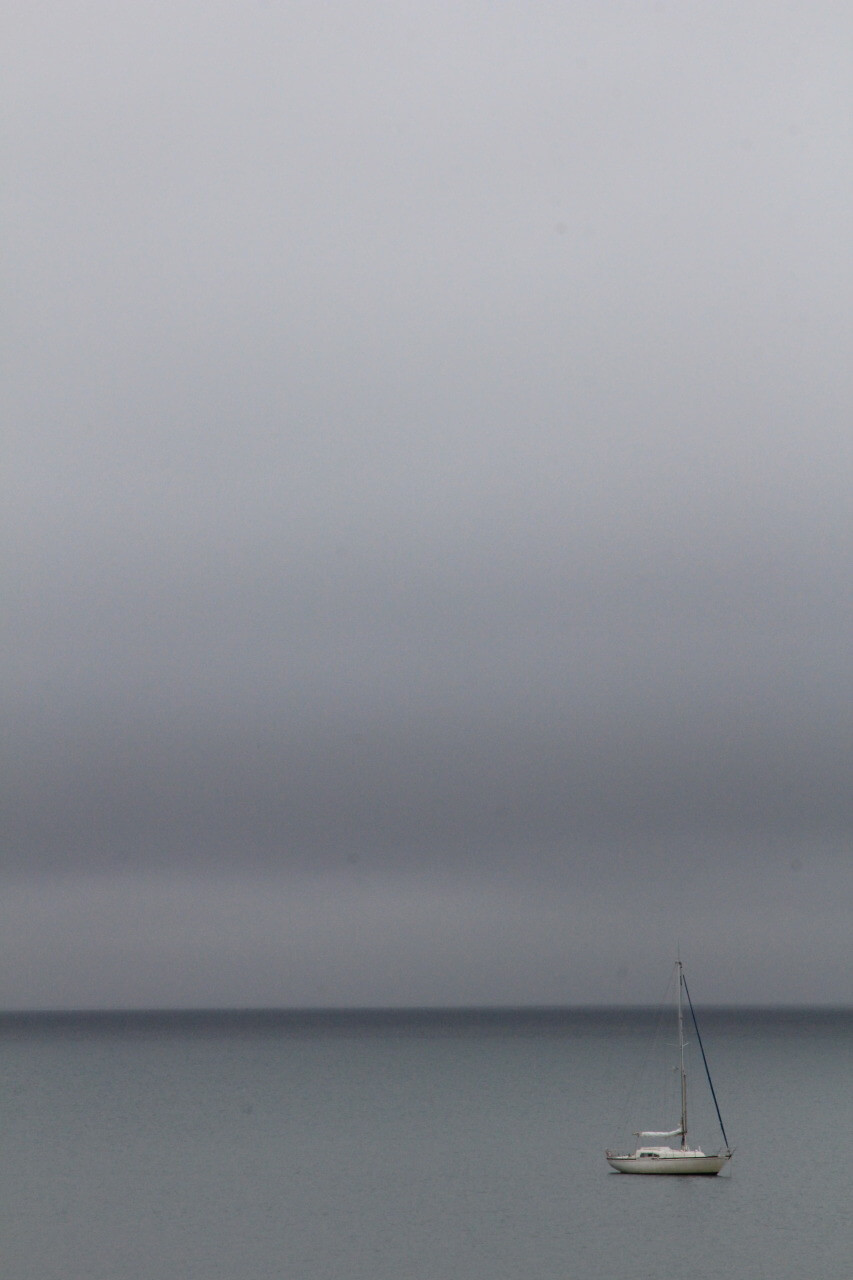
\includegraphics[width=0.4\textwidth, height=5cm, keepaspectratio]{../Bilder/Bretagne/6.jpg}
    \caption{Stimmung im Hafen}
  \end{centering}
\end{wrapfigure} 

Die ersten m�den Augen wurden erst um 10:30 ge�ffnet.
Die gestrige Fahrt war anstrengender als zuerst gedacht und der lange Schlaf war n�tig.
Nach dem einchecken auf dem Campingplatz und einem kurzen Besuch des Shops ging es ans erste Fr�hst�ck.
Schon w�hrend dem Fr�hst�ck ging der Triathlon in seine n�chste Runde.
Fahrer aller Kategorien strampelten am Campingplatz vorbei.
Das Wetter verhiess heute leider nichts gutes, es nieselte ganz fein.
So war alles in ein dumpfes grau eingepackt.
Unsere Fahrt ging zuerst gegen den Uhrzeigersinn um die Insel Richtung Port Haliguren wo wir so gleich f�r das Abendessen in einer wundersch�nen kleine Creperie reservierten.
Danach fanden wir den \glqq Boucle de Quiberon\grqq{} ein ausgeschilderter Fahrrad-Rundweg rund um Quiberon.
Wir folgten diesem und fanden uns in mitten von kleinen D�rfer wieder.
Unser Ziel die \glqq Cote Sauvage\grqq{} fanden wir schon bald und wanderten der wundersch�nen wilden K�ste entlang.
Unter dem \glqq Point de Percho\grqq{} waren viele Surfer im Meer welche im k�hlen Wasser die anst�ndigen Wellen genossen.
Bilder wurden gemacht und bald darauf meldete unser Bauch sich und verlangte nach etwas zu beissen.
Da die Zeit schon ziemlich Fortschritten war ging es direkt nach Quiberon zur�ck f�r einen Ap�ro.
In der selben Bar wie am ersten Tag genossen wir was zum trinken und die umfangreiche Ap�ro Platte dazu.
Dann hiess es noch einmal in die Pedalen zu treten um dann in der Creperie \glqq Du Vieux Port\grqq{} einen Fischsalat, Muscheln und einen in �l eingelegten Fisch zu geniessen.
Wobei der �l-Fisch nicht gerade f�r Begeisterungsst�rme gesorgt hat.
Die schlechte Wahl wurde umgehend mit einem Cr\^{e}pes kompensiert.
Auch ich kam nicht an solch einem Teig-Fladen vorbei und so wurde ein weiteres Mal Alkohol w�hrend dem Flambieren in W�rme umgewandelt.
Die kurze Fahrt zur�ck zum Camping verging im Flug und schon bald schlummerten zwei friedlich im VW Bus.

\begin{figure}[H]
   \centering
      %\subfloat[CAPTION]{BILDERCODE}\qquad
   \subfloat{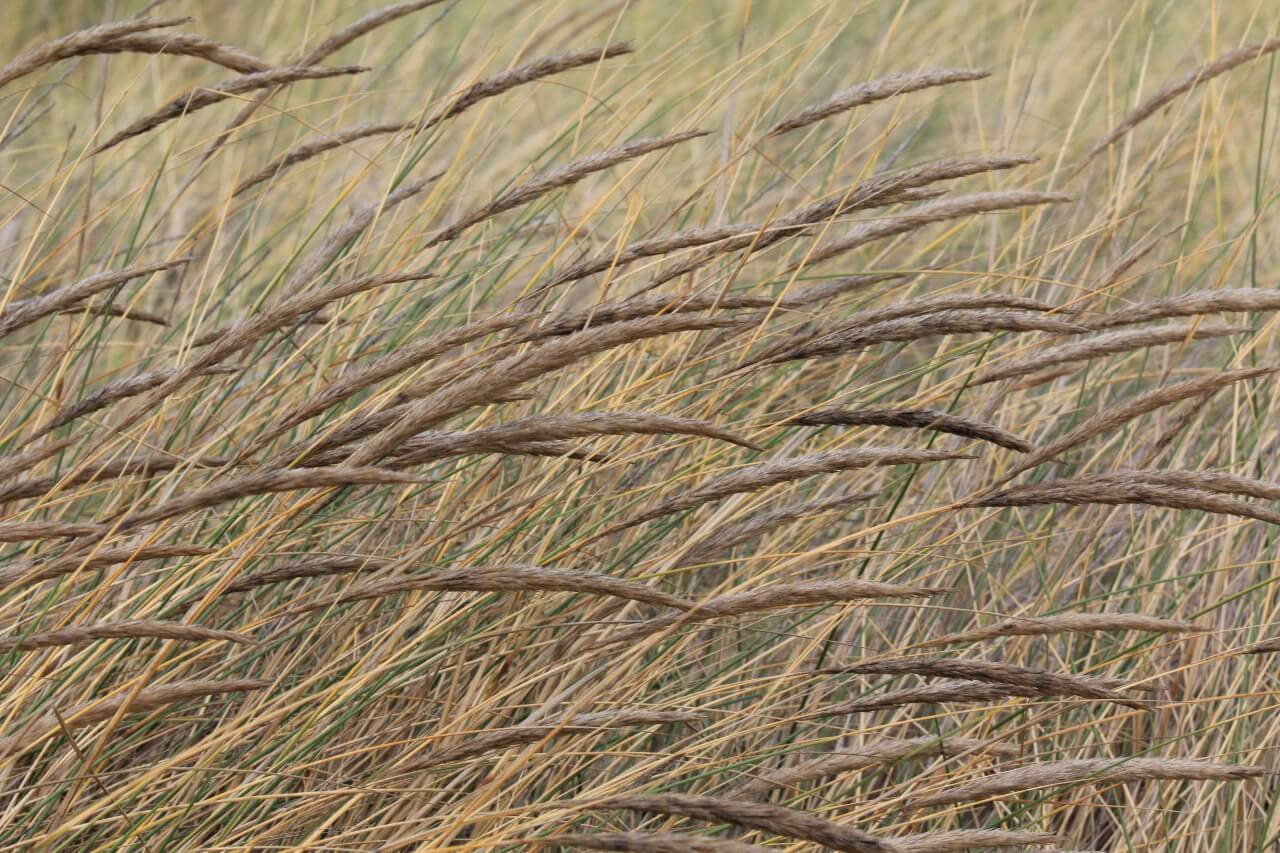
\includegraphics [width=0.3\textwidth]{../Bilder/Bretagne/10.jpg}}\quad
   \subfloat{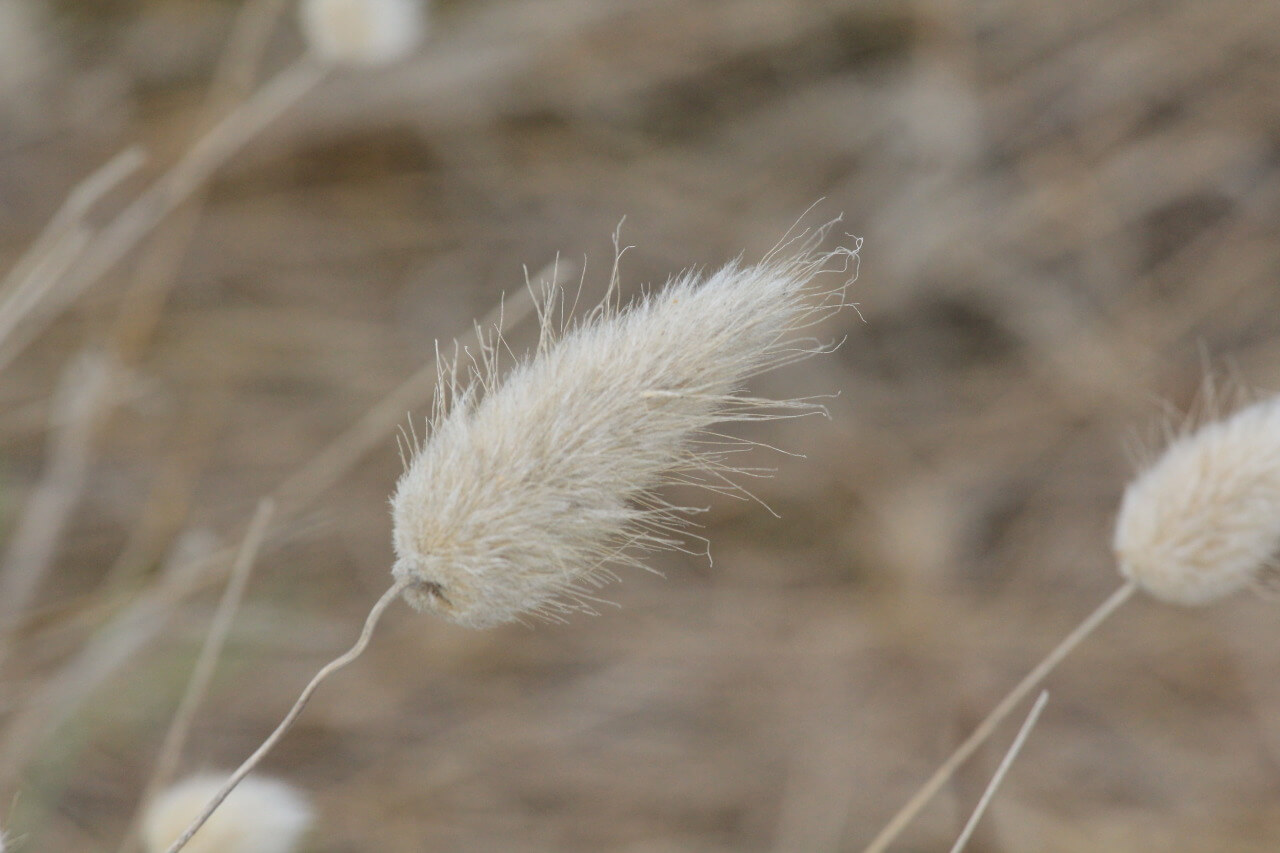
\includegraphics [width=0.3\textwidth]{../Bilder/Bretagne/11.jpg}}\quad
   \subfloat{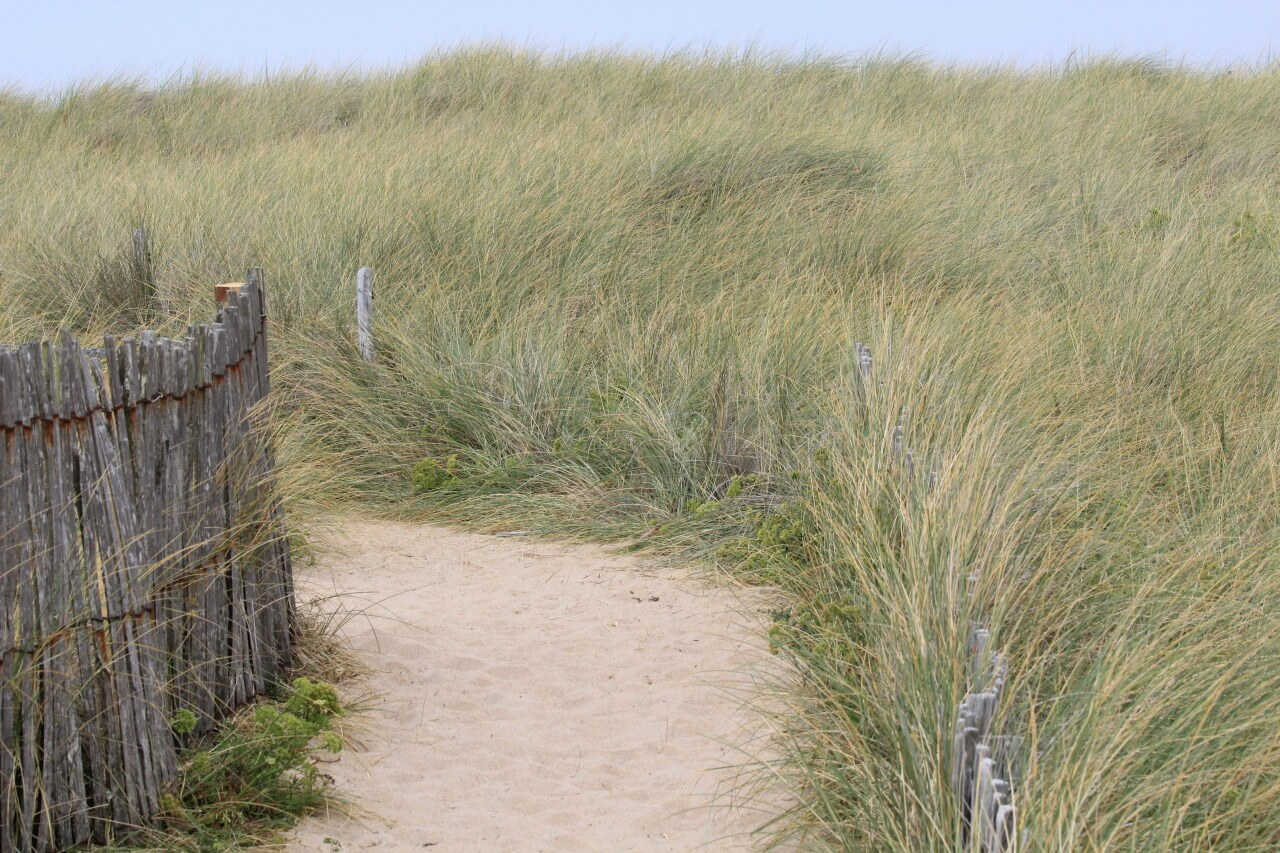
\includegraphics [width=0.3\textwidth]{../Bilder/Bretagne/12.jpg}}\quad
   \caption[Quiberon]{Quiberon}
\end{figure}

\subsection{05.09.2016 Der K�ste entlang}
Trotz einer Flasche Cider am Vortag, standen wir schon um 8:30 auf.
Naja waren immerhin wach.
Ein leises Tropfen verhiess nichts gutes und die Stimmung der besseren H�lfte sank unter Null.
Diese hob sich erst nach dem Fr�hst�ck im Bus! 
Kurz vor 11:00 fuhren wir los Richtung \glqq Auray\grqq{}.
Wieso das? Ganz einfach wir konnten bei der Fahrt nach Quiberon bereits einen Blick auf das Dorf werfen und es machte Eindruck.
Die Fahrt bei die Halbinsel verlief zuerst schleppend, da es hier immer Stau zu haben scheint.
Kurz darauf fanden wir dann in Array einen Parkplatz (Merci ihr Briten f�r das saubere queuing).
Genau heute fand ein Markt statt und dieser Umstand kombiniert mit dem besseren Wetter steigerte die Laune auf ein neues Allzeithoch.
Die Stadtbesichtigung wurde mit einem Besuch einer Creperie beschlossen und schon ging es weiter alles Richtung Lorriot.
Wir wollten nicht den ganzen Weg auf der Schnellstrasse verbringen und so bogen wir nach Lorriot mittels einiger Umwege zum Fort Bloqu� ab.
Dort bestaunten wir den kilometerlangen Sandstrand und die w�rmende Sonne.
Jetzt trennten uns nur noch unz�hlige Kreisel vom heutigen Etappenziel \glqq Concorneau\grqq{}.
Der Campingplatz wurde nach einer Navigon Irrfahrt gefunden und war leider voll\dots{}  wobei es fand sich noch ein \glqq kleines\grqq{} Pl�tzchen welches keine Parzellen hatte.
Wir nahmen dankend an und installierten uns auf der Wiese.
Schon beim Einchecken wurden wir im breitesten Bernerdialekt angequatscht und willkommen geheissen.
Ein Vertreter des VW-Bus Club der Schweiz war auch auf dem Campingplatz.
Die restlichen L�tstellen der schlampig gemachten Verbindung quittieren auch noch ihren Dienst und wollten repariert werden, was sogleich in Angriff genommen wurde.
Nach dem Aufstellen auf der ausladenden Wiese besuchten wir das Camping-Restaurant, in welchem uns zum wiederholten Male klar gemacht wurde, dass unser Franz�sisch nur m�hsam ist.
Nach den ersten Brocken der komplizierten Sprache wurde sogleich auf Englisch gewechselt.
Der Fisch, den Chantal serviert bekam war wunderbar und mein Entrecote konnte sich auf jeden Fall auch sehen lassen.
Der bestellte Wein tat seinen Teil und schon bald verzogen wir uns in den Bus.
Gerade als wir zum Platz zur�ck kamen, parkten zwei �bergrosse Italienische Wohnmobile auf der Wiese neben dem Bus.

\subsection{06.09.2016 little Dubrovnik}
Beim ersten Blick aus dem Bus war nur blauer Himmel zu sehen.
Das sch�ne Wetter motivierte zum Aufstehen, dieses wurde jedoch trotzdem auf sp�ter verschoben.
Als dann schlussendlich die T�ren ge�ffnet wurden, war der Himmel schon wieder mit feinen Wolken �berzogen.
Die bestellten Br�tchen wurden abgeholt und es wurde an der Sonne gefr�hst�ckt.
Der kurze Spaziergang nach Concorneau verlief durch ein Wohnquartier und danach immer der Nase lang.
Das durch eine sch�ne Stadtmauer eingeschlossene St�dtchen erinnerte stark an Dubrovnik, einfach im Massstab 1:2.
Auch hier war es m�glich die Stadt auf der Mauer zu umrunden.
Neuank�mmlinge w�rde durch eine keltischen Live Band begr��t und die Hauptstra�e war ges�umt mit Souvenir Shops.
Nach dem ersten erkunden der Stadt fanden wir etwas abseits eine Creperie bei welchen wir das Bretonische Standardmen� (Moule und Cr\^{e}pes) verdr�ckten.
Die Stadt ist zwar relativ touristisch, besticht jedoch durch die Befestigungsanlage im Wasser und der sch�nen K�ste.
Der Spaziergang dem Meer entlang Richtung Sable Blances war wundersch�n und der Strand machte Lust auf einen Tag Faulenzen.
Zur�ck auf dem Camping verl�ngerte ich unseren Aufenthalt um eine Nacht und genossen das sch�ne Wetter am Pool.

Wir waren uns schnell einig, dass wir es bei dieser Reise nicht bis nach Belgien schaffen werden und dass h�chstwahrscheinlich auch die Normandie nicht dieses Jahr bereist wird.
Die Reiseziele laufen ja nicht davon und wir m�chten die Bretagne nicht einfach Durchreisen damit wir da gewesen waren.
So wurde St. Michel als neues Ziel gesetzt.
Das Nachtessen nahmen wir ein weiteres Mal im Camping-Restaurant ein, welches sich schon am Vorabend als gute Adresse erwiesen hat.

Um mich auf die Bretagne einzustimmen hatte ich mir ein Krimi von Failler heruntergeladen und an diesem Abend noch fertig gelesen.
Nette Geschichte aber leider auch nicht mehr.


\subsection{07.09.2016 Beach Day}
Heute war Strandbad angesagt! Lesen, Sonne, Sand und Wasser und alles bei bestem Wetter an der Sable Blanc.
Der m�ssige Wind am Strand lud f�rmlich zum Drachenfliegen ein.
So sollte es geschehen.
Der Tag verging wie im Fluge und wurde nur durch ein feines Mittagessen (nein, ausnahmsweise keine Muscheln oder Cr�pes, sondern Fisch mit Curry Reis, herrlich diese Abwechslung) unterbrochen.
Nach dem wir so richtig gar gebraten waren, ging es zur�ck auf den Camping f�r eine erfrischende Dusche, so dass nachher bei einem wunderbaren Sonnenuntergang der Weg nach Concorneau unter die Pedalen genommen werden konnte, um weitere Teig-Fladen in der Stadt zu verdr�cken.

\subsection{8.09.2016 Quimper und Pointe de Raz}
Diese Nacht war kalt, sehr kalt.
Dank dem klaren Himmel ging die Temperatur Richtung einstelligen Bereich.
Um Chantal um 8:00 aus dem Schlafsack zu bringen, bedurfte es schon �berredungsk�nste eines Versicherungsvertreters.
Gl�cklicherweise hatte ich mit der Standheizung noch ein Ass unter dem Bus.
Die Heizung r�hrte los und schon bald war es im Bus wohlig warm.
Kurz nach halb zehn verlie�en wir den Camping und fuhren Richtung Quimper.
Auch dieser Weg war mit lauter Kreisel bespickt, welche alles andere als dienlich f�r den Fluss der Fahrt waren.
Kurz vor Quimper f�llten wir unsere Vorr�te in einem Super March� auf (endlich Batterien).
Mittels Navi fanden wir nach kurzer Zeit den Parkplatz in Quimper und schlenderten Richtung Kathedrale.
Bilder geschossen, die sch�nen H�user betrachtet und nach einem Caf� zog es uns schon bald weiter Richtung Point Raz.

Grosser Tourismus empfing uns an der K�ste.
Es gab sogar Shuttle-Busse welche die lahmende Touristen vom Parkplatz bis ganz zur K�ste fuhren.
Wir nahmen diese Meter jedoch wieder gerne unter unsere Sohlen und fanden uns dann schon bald an der wilden K�ste am westlichen Zipfel von Frankreich wieder.
Unz�hlige oder doch eher �berz�hlige Fotos wurden geschossen und meine obligatorischen M�wen Portrait wurden auch abgelichtet (brauche doch einen neuen Desktop-Hintergrund).
Nach einer Stunde Kraxlerei �ber Stock und Stein machten wir uns auf den R�ckweg zum Auto.
Auf dem Parkplatz angekommen liess sich Chantal zuerst einmal von der f�r sie �berw�ltigende Anzahl von Touri-Geschenken �berrumpeln.

Unser heutiges Etappenziel sollte der Camping Trez Rouz auf der Halbinsel Crozon sein.
Alles Tip Top ins Navi eingegeben und los konnte die wilde Fahrt gehen.
Doch nach zehn Minuten hatte ich die Schnauze voll.
Der erlektronische Helfer machte sich vermutlich einen Spass daraus uns �ber m�glichst m�hsame Strassen zum Ziel kommen zu lassen.
Garagen-Einfahrten, Fussg�ngerzonen und Fahrradwege waren heute die bevorzugte Routenwahl des kleinen Mistdings.
Darum ignorierte ich alle Bitte Wenden und jetzt abbiegen Aufforderungen und fuhr zur�ck auf ein Weg, der den Namen auch verdiente.
Schon bald wurden wir durch einen Fahrsch�ler im Lastwagen ausgebremst.
Habe ich schon erw�hnt, dass es doch einige Kreisel in der Bretagne gibt?
Die Kombination von ungewohnt grossem Gef�hrt und Kreisel gepaart mit Doppelkreisel plus ovale Kreisel liessen die Fahrtgeschwindigkeit auf ein neues Allzeittief sinken.

Wir kamen dann trotzdem noch auf dem Campingplatz an und stellten mit Freude fest, dass sich ein wundersch�ner Strand gegen�ber befand und das sich sogar ein Restaurant/Imbiss auf den Zeltplatz verirrt hat.
Mein Sitzplatz im Restaurant wurde von einer kleinen Katze bewacht, welche mir einen Schreck eingejagt hat.
Nach einem weiteren Cr\^{e}pe ging es in die Haia.

\subsection{Kleiner Nebenschauplatz}
Der Rasierer wurde bewusst zu Hause gelassen und durch ein Werbegeschenk (Cooles Teil, Sanyo, vollkommen aus Metall gefertigt) ersetzt.
Beim ersten Versuch am Sonntag Abend ist jedoch aufgefallen, dass die Batterien eher sehr leer waren und aus diesem Grund musste f�rs erste stolz mit einem spriesenden Bart die Ferien genossen werden.
Doch an diesem Geschichtstr�chtigen Tag sollte sich das Blatt wenden.

Da ich endlich frische Batterien f�r den Rasierer besorgt hatte konnte kurz nach Ankunft auf dem neuen Campingplatz mit dem Stutzen des bereist staatlichen Bartes begonnen werden.
Als Verst�rkung f�r den kleinen Werbegeschenk Rasierer von Waser, besorgte ich noch die guten alten Einweg Gillette Rasierer, welche mittlerweile auch schon mit drei Klingen aufwarten.
So bewaffnet ging es frohen Mutes in das Toiletten H�uschen.
Das kleine Ding surrte los und sogleich fielen die ersten Stoppeln in das Waschbecken, was ich mit einer gewissen Genugtuung zur Kenntnis nahm.
Der erste Blick in den Spiegel zeigte jedoch ein anderes Bild.
Die Reihen der Haare schien sich auch nach 5 Minuten kaum gelichtet zu haben, wie eine R�mische Legion setzten sie sich immer noch standhaft zu Wehr.
Ich gab dem Werbegeschenk noch einmal 5 Minuten Zeit um die Sache besser zu machen und tats�chlich zeigten sich erste Erfolge.
Wenn das so weiterging war ich bis Ende Ferien fertig rasiert.
Also den super Gillette Rasierer gez�ckt um die begonnene Schlacht ein f�r allemal oder eher die n�chsten zwei Tage zu gewinnen.
Leider war nach Einkauf kein Rasierschaum im Warenkorb und darum wurden die n�chsten 5 Minuten eher h�sslich und kratzig.
Nach dem Ende der Schlacht ging ich leicht blutend zur�ck zum Bus und �freute� mich schon auf die n�chste Rasur mit dem Duo.

\subsection{09.09.2016 B�ro und Pointe de Pen Hir}
Heute wollten wir die Gegen mit dem Velo unsicher machen.
Doch zuerst liessen wir den morgen gem�tlich mit Faulenzen und Brosch�re designen vor�berziehen.
Unser Platznachbar (mit einem wundersch�nen blauen Multivan T3) schaute nach einem Besuch auf jackthebus.com f�r ein kurzes Gespr�ch bei uns auf.
Pointe de Pen Hir war zwar nicht gerade weit, der Wind (insbesondere der Gegenwind) sorgte jedoch f�r ein eher schweres Vorankommen.
Nach einigem Pedalen sind wir dann doch noch angekommen und freuten uns der sch�nen Aussicht, welche leider durch das sich zuziehende Wetter getr�bt wurde.

Der Nachmittag war schon fortgeschritten und ein leichtes Ziehen in der Magengegend k�ndigte Hunger an.
Cashew N�sse halfen kurz und schon bald hatten wir dank den N�ssen neue Freunde gefunden.
Drei M�wen gesellten sich mit der Absicht zu uns, auch einen Nachmittagsnack abzubekommen.
Nach vergleichsweise wenig Fotos ging es zur�ck Richtung Camaret.

Wir freuten uns auf den unterst�tzenden R�ckenwind und erwarteten eine leichte Fahrt.
Der R�ckenwind war da und half enorm, jedoch hielt uns ein Hungerast von k�rperlichen H�chstleistungen ab.
Es musste schnell etwas zum Beissen gefunden werden.
Im Fischerdorf gab es ein weiteres Mal eine unglaubliche Auswahl an Creperien.
Gl�cklicherweise hatte eine davon einen bretonischen Salat auf der Speisekarte, so das ich f�r einmal von den ja eigentlich gut schmeckenden Cr\^{e}pes verschont blieb.
Nach der R�ckkehr zum Bus verfiel Chantal in einen kommat�sen Nachmittagsschlaf und wollte so gar nicht mehr aufstehen.
Am Abend wollte ich selber kochen, auch wenn das Wetter nicht gerade dazu einlud.
Wieder einmal Pasta waren doch verlockend, auch wenn die Platzverh�ltnisse eher eingeschr�nkt waren.
Der Wein wurde mit jedem Glas (Becher --> Kaffeebecher) besser nach dem Abwasch wurden ein weiteres Mal fleissig Zeilen gelesen.

Doch leider lag schon bald ein unangenehmer Duft in der Luft.
Schr�g gegen�ber unserem Stellplatz, wurde die chemischen Toiletten der Campingmobile geleert und verstr�mten den Duft von verdautem und verwertetem Essen.

\subsection{10.09.2016 Es seicht wie bl�d}
Schon kurz nach dem ersten Blinzeln des Tages war klar, das mit dem Wetter wird heute nichts.
Ein richtiggehendes Rauschen war h�rbar und verhiess garantiert nichts gutes.
Das aller sch�nste daran: Heute wollten wir weiter --> Das heisst alles einpacken und vor allem Velos wieder auf dem Hecktr�ger montieren.
Sch�ne Aussichten wenn das Wasser schon in Pf�tzen auf der Wiese stand.
Nach kurzer Gegenwehr akzeptierten wir die Situation und Fr�hst�ckten zuerst einmal.
Dann hiess es Arschbacken zusammenkneifen und ab die Post.
W�hrend des zusammenr�umen wurde mir noch aufgezeigt, dass man das Aufstelldach bei anhaltendem Regen und Wind wohl besser schliesst.
W�hrend dem zusammenpacken regnete es ununterbrochen und wir waren froh, als wir unsere sieben Sachen im Bus verstaut hatten.

Heute sollte es zuerst nach Roscoff gehen.
Dies geschah auch reichlich unspektakul�r, w�hrend es wie aus Eimer k�belte.
In Roscoff angekommen lachte kurz die Sonne durch den bedeckten Himmel und wir schlenderten durch die Gassen von little Britain.
Ein h�bsches Fischrestaurant erk�mpfte sich mit Unterst�tzung des Magens unsere Aufmerksamkeit und schon bald sassen wir vor zwei fein duftenden Fischen.

Der Steg ins Wasser (what the fuck??) besuchten wir auch kurz und danach wollten wir zu unserem Etappenziel aufbrechen --> Ploumanach.
Sobald der Motor gestartet war, fing es wieder an zu tropfen.
Das Ziel war etwas ganz anderes als die Pl�tze welche wir bis jetzt besuchten.
Eher ein kleines Feriendorf als ein Campingplatz.
Daf�r bot der Platz jeden erdenklichen Luxus und befand sich an einem sehr sch�nen K�stenabschnitt.
Das Nachtessen liessen wie fast ausfallen (Pizza �ber die Gasse und eine feine Melone) Die Sonne zeigte sich auch wieder zwischen den kurzen Schauern.
Bald verschwanden wir f�r ein paar Minuten Film auf dem Tablet und weitere Zeilen im Buch in den Bus.
Die Temperatur sank schnell in sehr kalte Bereiche und die Standheizung wurde in dieser Nacht eingeweiht.
Irgendwann in der Nacht waren Klopfger�usche am Bus h�rbar.
Ob sich da jemand an den feinen T�nen der Standheizung aufregte oder ob eine M�we unseren Abfallsack an pickte werden wir wohl nie erfahren.

\subsection{11.09.2016 Jagd nach Macareux}
Nach einem sp�ten Aufstehen arbeitete Chantal an ihrer Brochure w�hrend dem ich den Abwasch erledigte und nachher mit der Idee f�r einen Bootsausflug zu den Sept Iles stolz zur�ck kam.
F�r die Mittagsverpflegung wollte ich selber sorgen und so kredenzte ich aus den Restbest�nden im Bus einen Thunfischsalat.

Die 2.5 st�ndige Bootstour mit Zwischenhalt auf der Insel �le aux Moines sollte um Viertel vor Vier vom nahe gelegenen Strand des St�dtchens Perros-Guirec losgehen.
Die Velos erwiesen uns ein weiteres Mal ihren Dienst und schon bald sassen wir an der Strandpromenade und schl�rften zufrieden einen Ap�ro.
Nach dem Umtausch der auf dem Campingplatz gekauften Gutscheine zu Tickets, ging es an Bord de Bootes welches haupts�chlich mit �lteren Semester besetzt war.
Die Fahrtdauer zur ersten der Insel betrug ca. eine halbe Stunden und bald wurden wir von einem riesigen Schwarm M�wen begr�sst.
Eine Kolonie dieser Flugk�nstler besiedelte die Insel und sorgte so daf�r, dass der Gipfel wie von Schnee bedeckt zu ein schien.
Nach dem eindr�cklichen Start erwartetet ich eine solche Fortsetzung, was leider nicht der Fall war.
Bei den n�chsten Inseln waren leider nur noch vereinzelte V�gel zu sehen, gl�cklicherweise liess sich dann aber noch eine Robbe kurz sehen.
Der Besuch des Leuchtturms, welches eine der Insel kr�nte sowie die Ruinen eines Forts rundeten die Bootstour ab welche dann mit einer Vorbeifahrt an den roten Felsen zu ende ging.

Nach einem kurzen Stopp beim Bus ging unsere kleine Fahrradtour weiter Richtung Ploumanach wo in einem der wenigen Restaurant direkt am Strand gegessen wurde.

\subsection{12.09.2016 Es geht nach Osten}
Da wir am Vortag einen Blick auf die bekannten roten Felsen werfen konnten wollten wir die heuet besuchen.
Zuerst musste jedoch der ganze Karsumpel wieder in den Bus verladen werden.
Dem K�stenweg entlang war es ein sch�ner Spaziergang durch die Felsen, welche sich sehr f�r kurze Kletterausfl�ge eigneten.
Unterwegs ist der Autofokus der Kamera leider teilweise ausgestiegen, trotz allem wurden ein weiterers Mal unz�hlige Fotos geschossen.
Dieser sch�ne K�stenabschnitt zog jedoch verst�ndlicherweise sehr viele Leute und Cars an uns so war es nicht vewrwunderlich, dass in Ploumanach alle Restaurant zum bersten voll waren.
Wir beschlossen im Bus zu essen und machten uns auf den R�ckweg.
�berhalb des Campingplatzes befand sich ein Parkplatz mit sch�nster Aussicht auf die Sept Iles.
Eine weitere strube Fahrt (� la Navigon... scheint irgendwie Tagesformabh�ngig zu sein) nach Paimpol sp�ter suchten wir den Campingplatz.
Es gab jedoch eine leichte Unstimmigkeit: Die Angegebene Distanz konnte irgendwie nicht stimmen, laut Reisef�hrer waren es 5 Kilometer von Paimpol bis zum Campingplatz.
Das Navi machte 10 daraus.
Naja, es wird doch sicher eine Abk�rzung geben.
H�tten sie wohl gerne.
Also Plan�nderung --> Kurz nach der Dorfausfahrt befand sich noch ein anderer Platz.
Den halt angesteuert.
Die Rezeption hatte noch � Stunden geschlossen, die Zeit wurde sinnvoll f�r nichts tun eingesetzt.
Chantal steuerte schon zielsicher auf einen Stellplatz zu und so wurde der Platz 86 f�r eine Nacht zu unserem Territorium.
Nach der erfrischenden Dusche war uns schnell klar, dass wir hier auf einem Art Altersheim Camping gelandet sind.
Beide unsere absolvierten Lebensjahre addiert w�rden bei weitem nicht f�r die angeh�uften Lebensjahre eines Nachbars reichen.
M�ssen wohl alles franz�sische Veteranen sein, welche aktiv in einem der beiden Weltkriege gek�mpft haben.
Apropos Kampf: Alle Franz�sischen Rentnerpaare vom Typ Krampfader Geschwader hatte als Zierde und Hobby mindestens einen Vierbeiner bei sich.
Gr�sse und Form unterschieden sich jedoch massiv und so konnte sich niemand so richtig vorstellen, dass da irgendwann vor langer Zeit ein gemeinsamer Vorfahr gewesen sein muss.
Als ich gerade von der Dusche kam, war der Platz von nerv�sem franz�sischen Geschrei eingedeckt.
Der Grund daf�r: Ein Wolfs�hnlicher schwarzer Hund wollte gerade eine kleine Trottoirmischung zur Vorspeise verdr�cken, was dessen Besitzer zu wilden Gefuchtel und Geschrei veranlasste.
Gleichzeitig fluchte das Herrchen des Hobby-Wolfes auf den kleinen Hund mit Anhang ein.
Nach zwei, drei nerv�sen Minuten war der ganze Spuck vorbei.
Daf�r sorgte das Belgische P�rchen mit lauten Schnarchger�uschen f�r eine neue Soundkulisse.
Die Nacht kann ja heiter werden.

Da ich aus Prinzip nur eine kleine Tasche mitnehmen wollte, gingen trotz Sparmassnahmen meine Kleider zu neige.
Mit anderen Worte; B�h, ich musste waschen.
Die Waschmaschine war schnell gefunden und schon bald hingen �ber dem Platz 86 Kleidungst�cke, Tibetischen Gebetsfahnen nicht un�hnlich.
M�glicherweise bes�nftigt dieses Religi�se Zeichen die aufgeregten Vierbeiner.

Die kurze Fahrt mit dem Fahrrad nach Paimpol wurde dort mit einem sehr feinen Nachtessen unter freiem Himmel belohnt.

\subsection{13.09.2016 In den D�nen}
Heute �durfte� Chantal wieder einmal Jack durch die Bretagen jagen.
Auf dem eher kuriosen Campinplatz herschte rege Aufbruchstimmung und von jeder Seite rollten die f�r die Region so typischen �bergrossen Caravans auf den Ausgang zu.
Meistens begleitet durch nerv�se Korrekturen der Gattinnen auf dem Beifahrerplatz.
F�r einmal suchte unser elektronische Helfer eine Route heraus welche durchaus Sinn ergab.
So ging esch sehr schnell Richtung Cap Fr�hel.
Das Wetter war ein weiters Mal sehr durchzogen, bretonisch eben oder bei uns w�rden wir Aprilwetter sagen.
Regen und Sonne wechselten sich unregelm�ssig ab und als wir beim Camping angekommen waren, fing es sogleich an zu Gewittern.
Der riesige nicht in Parzellen aufgetrennte Campinplatz direkt am Meer verf�gte noch �ber mehr als genug Platz und schon bald parkten wir den Bus und machten zuerst einmal eine Pause um den schlimmsten Regen abzuwarten.
Die Sonne meldete sich dann umso st�rker zur�ck und wir genossen den Rest vom Tag am Strand mit lesen, sehr kurzen Versuche ins Wasser zu h�pfen und Faulenzen.
Da sich dieser Camping nicht gerade in der N�he von Zivilisation befand, beschlossen wir selbst etwas zu Kochen.
Das dumpfe Grollen, welche das sanfte Wellenbrechen �bert�nte warnte vor einem neuen Gewitter.
Die arg geschrumpften Vorr�te, wollten wir eigentlich auf der Fahrt hierher noch auff�llen, das ging dann leider ein weiterers Mal unter.
Pasta waren ja absolut in Ordnung aber es war leider auch kein Wein mehr an Bord.
So beschloss ich um Viertel nach Sechs auf mich auf die Suche nach etwas trinkbaren zu machen.
Im Umkreis von 3 Kilometern wusste der Kollege nichts von einer Einkaufsm�glichkeit.
Mit dem Fahrrad ging es ins nahegelegene Dorf, Weiler, Haus.
Das sah alles eher nach Geisterstadt aus als nach Einkaufen.
Im Nachbardorf sollte sich March� U befinden.
Der muss um diese Zeit noch offen haben.
Frohen Mutes begab ich mich auf den Weg dorthin.
Leider eine Niete.
Geschlossen war das Ding.
Nach � h sinnlosen Geradel kam ich Pflotschnass (kein Regen aber sehr warm und feucht hier) zur�ck beim Bus an und ging erstmals unter die Dusche.
Mir kam noch in den Sinn, dass ich eine Flasche Cidre (eigentlich als Mitbringsel) im Bus hatte und die wurde umgehend k�hl gestellt.
Nach dem Abendessen wurden wir von einem Hasen besucht und die Flasche leerte sich schneller als einem lieb war.
Die Temperaturen waren weiterhin angenehm und ein wundersch�ner Sonnenuntergang kr�nte diesen Tag.
In der Nacht wurden wir durch Blitz und Donner geweckt und der Himmel �ffnete seine Schleusen und wusch die gesamte W�rme aus dem n�chtlichen Himmel.

\subsection{14.09.2016 Wo befinden sich hier die L�den}
Nach einem eher bescheidenen Fr�hst�ck stand nun deng�ltig fest, dass die Vorr�te aufgefrischt werden m�ssen.
Der Besuch des Cap Frehels stellt da gerade eine gute Gelegenheit dar, da wir sowieso mehrere D�rfer mit dem Fahrrad durchqueren mussten.
Die meisten angesteuerten Ladenlokale sahen sich dann aber zum verwechseln �hnlich:
Die zwei vorgefundenenen Kategorien:

Geschlossen weil heute ein Wochentag ist
Zu Verkaufen

bretagne 112 20160919 1366953728Wir beschlossen die Suche auf dem R�ckweg zu intensivieren und steuerten tapfer weiter auf das Cap Frehel zu.
Die Vorbeifahrt an einem Bistro liess den Magen grummeln und so wurde sofort der Blinker gesetzt und abgebogen.
Nach den besten Muscheln der Bretagne, Lachs mit Kartoffel und einem unglaublichen Dessert ging es weiter Richtung Leuchtturm, der schon von weitem sichtbar ist.

Nach dem obligatorischen erklimmen der Turmspitze war auch schon das Fort la latte in der Ferne sichtbar.
Ein Weg f�hrt der K�stenlinie entlang bis zu der Festung.
Frisch gest�rkt musste dieser Weg begangen werden.
Wundersch�ne Ausblicke in verschiedene Buchten belohnten das Unternehmen und auch das Fort war fast immer zu sehen.
Es wollte jedoch nicht so recht n�her kommen.
Auf einmal huschte ein kleines Fellkn�uel �ber den Weg und blieb am Rand bewegungslos stehen.
Eine kleine Maus.
Das tapfere Ding hatte �berhaupt keine Scheu und liess sich den Grashalm schmecken, welche ich ihr hinhielt.
Schlussendlich standen wir vor der Kasse der Burg und erkauften uns Zutritt.
Das sehr gut erhaltene (renovierte) Fort ist nett anzusehen, leider hapert es hier mit der Verpflegung.
So ging es den gleichen Weg zur�ck, jedoch betr�chtlich schneller, da die vielen Fotostopps ausgelassen wurden.
Ein weiteres Mal das Web nach Einkaufsm�glichkeiten in Fahrraddistanz durchforstet und die Recherche ergab eine M�glichkeit in Frehel.
20 Minuten sp�ter sind wir da angekommen und mussten ein weiteres Mal feststellen, dass es hier gar nicht so einfach ist etwas offenes in dieser Jahreszeit zu finden.
Bei der letzten M�glichkeit hatten wir jedoch Gl�ck und konnten uns mit dem wichtigsten eindecken.
Dem Abendessen stand nichts mehr im Weg und schon bald konnten wir einenm weiteren sch�nen Sonnenuntergang beiwohnen.
Chantal konnte sich mit dem Wein anfreunden und schlief schon bald im Bus :)

\subsection{15.09.2016 Party vor dem Hotel}
Leider mussten wir heute weiter.
Die sch�ne Aussicht, der Nahe Strand und die interessanten Landschaft h�tten dazu eingeladen ein bisschen l�nger zu bleiben.
Da sich jedoch eine Wetterverschlechterung ank�ndigte und es sich in St. Malo mit den Campingpl�tzen �hnlich verh�lt wie mit Einkaufsm�glichkeiten in Frehel, beschlossen wir f�r die restlichen Tage ein Hotel zu beziehen.
Die zuerst aufgerufenen waren leider voll, doch schon bald liess sich eines finden, welches sich nicht im Stadtzentrum befand, was der Parkplatzsuche (Mit Paulchen am Bus) sicher zu Gute kam.
Ein Anflug von unfassbarem Gl�ck bescherte uns ein Parkplatz direkt vor dem Hotel.
Die Lobby sah ganz vern�nftig aus, was auf das Zimmer nur beschr�nkt zu traf.
Rote Leder Kissen auf dem Bett und die dazu passenden roten Leder-Vorh�nge trafen nicht gerade auf Gegenliebe.
Zu dem war das Zimmer noch fast kleiner als der VW-Bus.

Wir waren ja nicht wegen dem Zimmer gekommen und so machten wir uns auf dem Weg in die Stadt.
Alles der sch�nen Strandpromenade und dem breiten Strand entlang ging es fast 40 Minuten bis wir vor den Stadtmauer von St. Malo standen.
Sofort erkundeten wir die verschiedenen Gassen und Strassen und ich ging auf die Suche nach einem sch�nen Restaurant, w�hrend dem Chantal die Gesch�fte der Stadt unsicher machte.
Die Suche nach einem Restaurant war absolut erfolgreich wie sich wenig sp�ter herausstellen sollte.
Ein Fisch Men� inklusive Weinbegleitung, herrlich.

Der Weg zur�ck ins Hotel kam gerade gelegen, um die Verdauungen etwas anzukurbeln und den Kopf nach einigem Alkohol auszul�ften.
Kurz bevor wir beim Hotel waren, trafen wie auf eine gr�ssere Truppe, welche auf der Promenade eine Party feierte.
Noch nicht einmal im Bett und lautes Prasseln war zu h�ren, welches durch starken Regen verursacht wurde.
Die Party-Meute suchte Schutz vor dem Nass und beschloss diesen Schutz lautstark vor unserem Hotel gefunden zu haben.

\subsection{16.09.2016 Wetter: Bretonisch}
Nach einer eher unruhigen Nacht, machten wir uns kurz nach halb zehn auf den Weg nach unten, um das Fr�hst�ck einzunehmen.

Das Wetter sah immer noch nach Regen aus, doch es regnete nicht.
Dick eingepackt ging es es Richtung St. Malo.
Kite-Surfer zogen ihre Bahnen vor dem Strand, welcher ein breites Band bis zur Stadt zieht.
Die frische Luft tat gut und gl�cklicherweise blieb es vorerst auch trocken.

Vor der Hafeneinfahrt von St. Malo befindet sich ein langer Schutzwall, welcher begangen werden kann.
Dies nahm ich mir als n�chstes Ziel vor.
Der heftige Seegang an diesem Morgen machte den Weg spannend.
Einzelne Wellen �berfluteten den Weg immer wieder.
Chantal genoss einen Kaffee w�hrend ich an der Spitze der Mauer ein bisschen verweilte bis die Sonne hinter den Wolken hervorblickte.
Als wir uns wieder trafen klarte das Wetter immer mehr auf und wir umrundeten die Stadtmauer eine weile.
Ein kurzer Abstecher zur

Insel �Le grand B� die Dank Ebbe trockenen Fusses erreichbar war liess die M�gen knurren und schon kurz darauf befanden wir uns ein bei unserer Lieblingsbesch�ftigung: Dem Essen.
So eine Stadtbesichtigung macht ganz sch�n M�de und aus diesem Grund beschlossen wir den Nachmittag mit d�sen zu verbringen.
Auf dem R�ckweg, entlang der breiten Strandpromenade, setzte eine richtige Rush Hour auf dem Wasser ein.
Der starke Wind zog immer mehr Surfer und Kitesurfer an und �ber den Strand.
Es. Um uns einen ausgedehnten Spaziergang zu ersparen war der Plan in der N�he des Hotels zu essen.
Beim Ausgang des Hotels wurden wir auf eine Traube filmender Menschen aufmerksam, welche ihr Handy Richtung Meer hielten.
Da wo vorher noch eine Promenade war ist jetzt Meer.
Nichts mehr zu sehen von dem breiten Strand.
Der erste schm�lere Teil der Promenade wurde vollkommen vom Wasser �bersp�lt und es w�re zu dieser Zeit nicht m�glich gewesen unserem gewohnten Weg zu folgen.
Die vor dem Hotel geparkten Autos (unter anderem unser Bus) wurden ziemlich unsch�n mit einer dicker werdenden Salzschicht �berzogen.
Erinnerungen an Korsika wurden wach.

\subsection{17.09.2016 Dinan, wundersch�ne Stadt im Hinterland}
Das Wasser peitschte noch immer �ber die Promenade, als wir uns aus dem Hotel aufmachten einen Tages Ausflug nach Dinan zu machen.
Fr�her im Jahr g�be es die M�glichkeit mit die Strecke mit einem Boot zur�ckzulegen.
Leider wird dieser Service nur bis Ende August angeboten und so musste unser Bus als Taxi herhalten.
Nach dem er die ganze Nacht mit Salzwasser geduscht worden ist, geht er sowieso neuerdings auch als Boot durch.
Nach dem die Scheiben vom gr�bsten Sand und Salz befreit worden waren verliessen wir St. Malo auf dem schnellsten Weg Richtung Dinan wo unsere fr�hliche Ausfahrt j�h durch ein Stau, ausgel�st durch einen Unfall gestoppt wurde.

Dank Navi war kurz darauf ein Parkplatz gefunden und schmale Gassen ges�umt von krummen H�usern warteten auf eine Entdeckung.
Auf einem steilen Weg hinunter zu dem Fluss �la Rance� ist Chantal irgendein Teil des Knies blockiert.
Die sonst so �blichen Witze �ber alte Leute waren an diesem Tag nicht mehr ganz so lustig.
Das Alter fordert seinen Tribut.
Nach dem Umrunden der Stadt auf der Stadtmauer wurde noch der Kirchenturm bestiegen.
Die k�rperliche Verfassung der Teilnehmer unserer Altersreise reichte knapp f�r den Aufstieg.
Als wir die steile Treppe vom Turm hinunterstiegen meinte eine doch eher �ltere Dame zu Chantal �Oui, ce n�est pas facile�.
Kam bei Chantal, die mit schmerzverzerrtem Gesicht die Treppe herunter humpelte nicht gerade gut an.
Das Dorf machte sich bald darauf bereit um einen Stadtlauf durchzuf�hren und wir beschlossen uns mit dem Bus wieder Richtung St. Malo zu begeben.
Schon auf der Hinfahrt fiel uns ein ungewohntes Ger�usch auf, welches sich auch jetzt wieder bemerkbar machte.
Das wurde f�rs erste ignoriert und der bekannten Bus Reiseparanoia zugeschrieben.

Das Abendessen wollten wir direkt an der Promenade in einem wirklich grossen und gut besuchtem Restaurant zu uns nehmen.
Der Weg dorthin stellte sich jedoch als schwierigerer als gedacht heraus.

Nach etlichen Sprints ins trockene konnten wir gerade neben den beiden K�chent�ren unseren Platz einnehmen und dem wahnsinnig gesch�ftigen Treiben zusehen.
W�hrend dem ganzen Nachtessen peitschten die Wellen an die Fenster des Restaurants.
Ein gelungener Abschluss unserer Ferien in der Bretagne.

\subsection{18.09.2016 Rauf auf den H�gel}
Auf dem selben Weg, den wir am Vortag Richtung Dinan benutzt haben ging es nun nach dem Fr�hst�ck Richtung Mont St. Michel.
Auch heute war wieder das komische Ger�usch zu h�ren und mir wurde immer klarer das hier irgendetwas im Argen sein muss.
Nach dem wir von einem �berm�tigen Parkplatzw�chter vom normalen Parkplatz zum Parkplatz f�r Wohnmobile verwiesen wurden (haben wir jedoch gekonnt ignoriert), haben wir den Bus auf dem riesigen Parkplatz geparkt und ich konnte nicht anders als dem komischen Ger�usch auf den Grund zu gehen.
Nach kurzer Zeit war klar, dass sich eine Z�nkerze gel�st hatte.
Ich war mir leider nicht sicher, ob wir einen passenden Schl�ssel dabei hatten.
Zus�tzlich machten die es die auf dem Paulchen montierten Velos nicht gerade einfacher an den Motor zu kommen.
So beschlossen wir zuerst den H�gel anzuschauen und den Motor etwas abk�hlen zu lassen.

Der eindr�ckliche H�gel mit der aufgesetzten Abtei war dank dem Shuttle Bus schnell erreicht.
Unsere Gl�cksstr�hne hielt weiter an und genau heute war der Eintritt kostenlos.
Nach einer Runde durch die alten Gem�uer ging es zur�ck zum Bus um die Kerze anzuziehen.
Leider gewann die Faulheit und aus diesem Grund wurde die Bank nicht zur�ckgelegt um an das Werkzeug unter der Bank zu kommen.
So musste eine Spitzzange reichen um die Kerze wieder (ein bisschen) fest zu ziehen.
Eine H�rprobe best�tigte den Erfolg des Quickfix.

Der Weg zur�ck in die Schweiz mit open end verlief absolut problemlos.
Da wir erst kurz vor Mittag abgefahren waren, war es klar das wir die Strecke nicht an einem St�ck fahren wollen.
Kurz nach Mitternacht standen wir vor unserem Zuhause in Luzern.
Die Fahrt ging so gut, dass nie der Wunsch nach einer l�ngeren Pause aufkam.

\subsection{19.09.2016 Aufr�umen beginnt}
Nach der weiten Reise hatte es unser Bus verdient wieder richtig sauber gemacht zu werden.
Das wurde in der Woche nach unseren Ferien erledigt.
Die meisten bekannten M�ngel wurden noch behoben (Z�ndkerze).
Der zugeh�rige Schl�ssel w�re auf jeden Fall mitgef�hrt worden.

Nach der wundersch�nen Reise ist wurde VW Bus ein weiteres Mal als Werkzeug Transporter gebraucht und danach f�rs erste in die Tiefgarage zur�ckgestellt.

\newpage

\begin{figure}[H]
    \centering
    
\includegraphics[width=\textwidth,height=14cm, keepaspectratio]{../Bilder/Logo/Logo_trans.png}
    \label{img:Logo}
\end{figure}
\vfill
    \begin{center}
        {\huge  Weitere Informationen zum Bus und unseren Reisen sind auf der Homepage {\url{www.jackthebus.com}} zu finden}
\end{center}

\end{document}
